\section{Реализация}

На рис.~\ref{fig:impl_stages} представлена схема последовательности разработки библиотеки \texttt{cast-castle}, отражающая ключевые шаги от анализа требований до тестирования.

\begin{figure}[H]
    \centering
    
\includegraphics[width=1.0\textwidth]{images/diagrams/Этапы реализации.png}
    \caption{Схема этапов реализации библиотеки cast-castle}
    \label{fig:impl_stages}
\end{figure}

\textbf{Описание этапов (в соответствии со схемой):}

\begin{enumerate}
    \item Анализ требований и проектирование API – определение сценариев маппинга (прямое копирование, разные имена полей, вложенные объекты, коллекции, nullable-типы).
    \item Объявление аннотации \texttt{@CastCastleMapper} в модуле \texttt{annotations} – создание аннотации с целями \texttt{CLASS} и \texttt{FUNCTION}, удержанием \texttt{BINARY}.
    \item Настройка Gradle модуля \texttt{processor} – подключение KSP API, KotlinPoet, настройка зависимостей.
    \item Реализация точки входа – класс \texttt{CastCastleProcessorProvider} – фабрика для регистрации процессора через \texttt{META-INF/services}.
    \item Разработка компонента разрешения символов – \texttt{ComponentsResolver} – обход аннотированных элементов, классификация классов и функций, построение начальных моделей.
    \item Создание внутренних моделей данных – \texttt{ClassModel}, \texttt{Parameter}, \texttt{MapperClass}, \texttt{MapperMethod}, \texttt{ImplMapperClass} и т.д.
    \item Реализация рекурсивного анализа – методы \texttt{recursiveGenerateMapperCall()} и \texttt{generateCollectionMapping()} для обработки вложенных объектов и коллекций.
    \item Реализация генерации кода – класс \texttt{StringViewGenerator}, формирование функций с суффиксом \texttt{CastCastle} и добавление недостающих параметров.
    \item Реализация файлового вывода – класс \texttt{FileWriter}, запись сгенерированных \texttt{.kt}-файлов через \texttt{CodeGenerator} с указанием зависимостей.
    \item Интеграционное тестирование – написание и тестирование компиляции примеров (вложенные объекты, коллекции, дополнительные параметры, companion-объект) и проверка сгенерированного кода.
\end{enumerate}

Библиотека \texttt{cast-castle} состоит из двух модулей: \texttt{annotations} и \texttt{processor}. Модуль \texttt{annotations} содержит единственный файл \texttt{CastCastleMapper.kt} с объявлением аннотации. Модуль \texttt{processor} содержит реализацию KSP-процессора, разбитую на несколько пакетов и классов. Ниже приведено подробное описание каждого компонента.

\subsection{Диаграмма классов библиотеки cast-castle}

На рис. ~\ref{fig:class_diagram} представлена диаграмма классов разработанной библиотеки, отражающая структуру KSP-процессора и его взаимодействие с моделями данных.

\begin{figure}[H]
    \centering
    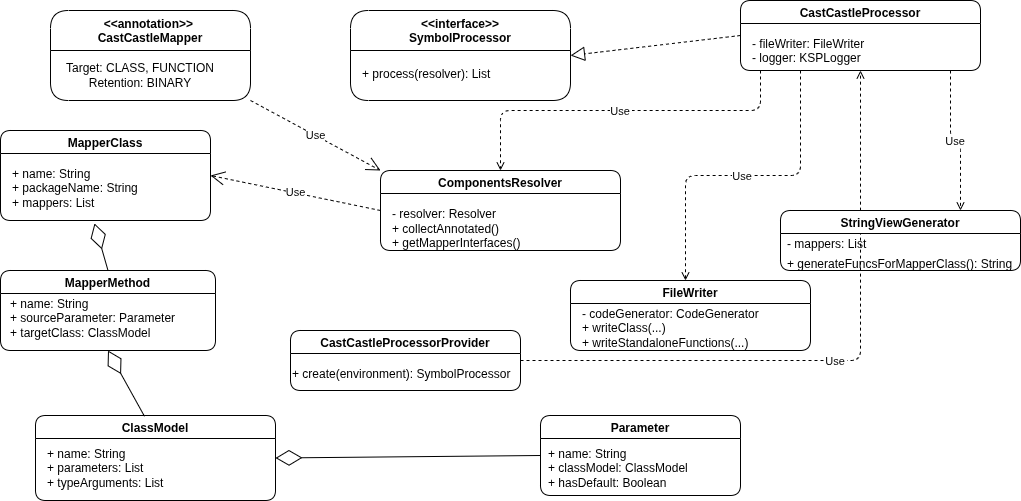
\includegraphics[width=1.0\textwidth]{images/diagrams/диаграмма классов.png}
    \caption{Диаграмма классов библиотеки cast-castle}
    \label{fig:class_diagram}
\end{figure}

\subsection{Модуль аннотаций}

Файл \texttt{CastCastleMapper.kt}:

\begin{lstlisting}
package ru.vafeen.castcastle.annotations

@Target(AnnotationTarget.CLASS, AnnotationTarget.FUNCTION)
@Retention(AnnotationRetention.BINARY)
annotation class CastCastleMapper
\end{lstlisting}

\textbf{Анализ:}
\begin{itemize}
    \item \texttt{@Target(AnnotationTarget.CLASS, AnnotationTarget.FUNCTION)} — аннотацию можно применять к классам (включая интерфейсы, классы-объекты, companion-объекты) и к функциям (включая функции-члены, функции расширения и standalone-функции).
    \item \texttt{@Retention(AnnotationRetention.BINARY)} — аннотация сохраняется в байт-коде, но не доступна в рантайме через рефлексию. Этого достаточно для KSP, который работает на уровне байт-кода, и при этом позволяет избежать загрязнения рантайма.
\end{itemize}

Других аннотаций в библиотеке нет — весь контроль осуществляется через единственный маркер.

\subsection{Модуль процессора}

Модуль процессора организован следующим образом (путь: \texttt{cast-castle-processor/src/main/java/ru/vafeen/castcastle/processor/}):

\begin{itemize}
    \item \texttt{CastCastleProcessor.kt} — главный класс процессора.
    \item \texttt{CastCastleProcessorProvider.kt} — фабрика процессоров для KSP.
    \item \texttt{processing/} — пакет с основной логикой:
        \begin{itemize}
            \item \texttt{ComponentsResolver.kt} — анализ аннотированных символов и преобразование их в модели данных.
            \item \texttt{FileWriter.kt} — запись сгенерированных файлов через \texttt{CodeGenerator}.
            \item \texttt{ProcessingVisibility.kt} — обработка модификаторов видимости (public/internal).
            \item \texttt{mapper\_generators/StringViewGenerator.kt} — генерация исходного кода в виде строк.
            \item \texttt{models/} — data-классы для представления моделей (\texttt{ClassModel}, \texttt{MapperClass}, \texttt{ImplMapperClass} и т.д.).
            \item \texttt{utils/} — вспомогательные функции: проверка коллекций, генерация имён, copyright.
        \end{itemize}
\end{itemize}

\subsubsection{Точка входа: CastCastleProcessorProvider и CastCastleProcessor}

Класс \texttt{CastCastleProcessorProvider} реализует интерфейс \texttt{SymbolProcessorProvider} — это стандартный механизм KSP для регистрации процессора. Файл с именем этого класса помещается в директорию \texttt{META-INF/services}, благодаря чему KSP находит процессор во время компиляции. В методе \texttt{create()} провайдер создаёт экземпляр основного процессора \texttt{CastCastleProcessor}, передавая ему генератор кода (\texttt{CodeGenerator}) и логгер (\texttt{KSPLogger}).

Главный класс \texttt{CastCastleProcessor} наследуется от \texttt{SymbolProcessor} и переопределяет метод \texttt{process()}. В этом методе происходит следующее:

\begin{enumerate}
    \item Создаётся экземпляр \texttt{ComponentsResolver}, который выполняет первичный обход всех аннотированных символов.
    \item Из резолвера извлекаются два списка: \texttt{interfaces} (аннотированные классы) и \texttt{standaloneFunctions} (отдельные функции, помеченные аннотацией).
    \item Для каждого класса генерируется отдельный выходной файл. Имя этого файла образуется добавлением суффикса \texttt{CastCastle} к исходному имени класса. Генерация делегируется \texttt{FileWriter} и \texttt{StringViewGenerator}.
    \item Для всех standalone-функций выполняется группировка по имени пакета. Для каждого пакета создаётся один файл \texttt{StandaloneFunctions.kt}, в который помещаются все сгенерированные вспомогательные функции этого пакета.
\end{enumerate}

Код процессора не содержит сложной логики ожидания (отложенной обработки) — все найденные символы обрабатываются сразу, а возвращаемый список пуст.

\subsubsection{Компонент разрешения символов: ComponentsResolver}

Класс \texttt{ComponentsResolver} отвечает за анализ исходного кода и преобразование низкоуровневых KSP-символов во внутренние модели данных. Его ключевые функции:

\begin{itemize}
    \item \texttt{collectAnnotated()} — получает через \texttt{resolver.getSymbolsWithAnnotation(...)} все элементы, помеченные \texttt{@CastCastleMapper}. Каждый элемент классифицируется:
        \begin{itemize}
            \item Если это класс (\texttt{KSClassDeclaration}), он преобразуется в \texttt{MapperClass}.
            \item Если это функция, у которой нет родителя-класса (то есть функция верхнего уровня), создаётся \texttt{MapperStandaloneFunction}.
            \item Если функция принадлежит классу, но сам класс не аннотирован, процессор выдаёт ошибку: родительский класс тоже должен быть помечен \texttt{@CastCastleMapper}.
        \end{itemize}
    \item Для класса дополнительно извлекаются все его функции, которые являются кандидатами в мапперы: функция должна иметь ровно один параметр и возвращаемый тип. Такие функции превращаются в \texttt{MapperMethod}.
    \item Для standalone-функции определяется исходный объект: если функция является расширением, то исходный объект — это приёмник (\texttt{this}); в противном случае — первый параметр. Возвращаемый тип считается целевым классом.
    \item Параметры конструктора целевого класса получаются путём анализа первичного конструктора (для Kotlin) или первого публичного конструктора (для Java). Это критически важно для правильной генерации вызовов конструктора.
\end{itemize}

Методы \texttt{getParameters()} и \texttt{toClassModel()} рекурсивно обходят структуру классов, включая generic-аргументы, что позволяет корректно обрабатывать вложенные типы и коллекции.

\subsubsection{Модели данных}

В пакете \texttt{models} определены data-классы, служащие унифицированным представлением анализируемой информации:

\begin{itemize}
    \item \texttt{ClassModel} — хранит имя, пакет, видимость, список параметров (полей) и generic-аргументы. Используется как для исходных, так и для целевых классов.
    \item \texttt{Parameter} — описывает отдельный параметр (поле) класса: имя, тип (\texttt{ClassModel}), наличие значения по умолчанию.
    \item \texttt{MapperClass} — агрегирует данные об аннотированном классе: его имя, пакет, список методов-мапперов (\texttt{MapperMethod}), видимость.
    \item \texttt{MapperMethod} — представляет функцию-маппер внутри класса: её имя, исходный параметр, целевой класс, абстрактность, наличие собственной аннотации.
    \item \texttt{ImplMapperClass} и \texttt{ImplMapperMethod} — модели для генерируемых классов и методов (содержат информацию, необходимую при построении выходного кода).
    \item \texttt{MapperStandaloneFunction} и \texttt{ImplMapperStandaloneFunction} — аналогично для отдельных функций.
\end{itemize}

Эти модели полностью отделяют логику анализа от логики генерации: \texttt{ComponentsResolver} заполняет модели, а \texttt{StringViewGenerator} затем использует их для создания текста.

\subsubsection{Генерация кода: StringViewGenerator}

Класс \texttt{StringViewGenerator} отвечает за превращение внутренних моделей в строки исходного кода на Kotlin.

Основные методы генератора:

\begin{itemize}
    \item \texttt{generateFuncsForMapperClass()} — создаёт реализации всех методов для сгенерированного класса.
    \item \texttt{generateStandaloneFunctions()} — создаёт вспомогательные функции для standalone-случаев.
\end{itemize}

\paragraph{Алгоритм для функции-маппера (\texttt{fun map(a: A): B}).}
\begin{enumerate}
    \item Из модели получается целевой класс \texttt{B} и список его параметров (полей).
    \item Для каждого параметра целевого класса проверяется, есть ли в исходном классе поле с точно таким же именем. Если поле найдено и типы совместимы, генерируется обращение вида \textbf{a.поле}. Если поле отсутствует — оно добавляется как параметр в сигнатуру генерируемой функции.
    \item Имя генерируемой функции образуется добавлением суффикса \texttt{CastCastle} к исходному имени (например, \texttt{map} → \texttt{mapCastCastle}).
    \item Тело функции представляет собой вызов конструктора целевого класса, в который передаются значения полей (из исходного объекта или из добавленных параметров).
\end{enumerate}

\paragraph{Рекурсивная обработка вложенных объектов.}
Метод \texttt{recursiveGenerateMapperCall()} вызывается, когда тип поля в исходном классе сам является сложным типом (другим классом или коллекцией). Алгоритм:
\begin{itemize}
    \item Проверяется, не возникла ли циклическая зависимость (с помощью множества \texttt{visitedTypes}); если да — генерируется заглушка \texttt{TODO("Circular mapping")}.
    \item Если тип поля — коллекция, управление передаётся в \texttt{generateCollectionMapping()}.
    \item В противном случае ищется прямой маппер между типами внутри того же класса. Если такой маппер найден, генерируется его вызов. Если нет — строится рекурсивный вызов конструктора для вложенного целевого класса (аналогично основному алгоритму).
\end{itemize}

\paragraph{Обработка коллекций.}
Метод \texttt{generateCollectionMapping()} определяет тип коллекции по имени класса (\texttt{List}, \texttt{Set}, \texttt{MutableList}, \texttt{ArrayList}, \texttt{HashSet} и т.д.). Затем:
\begin{itemize}
    \item Извлекаются типы элементов для исходной и целевой коллекции (через \texttt{typeArguments}).
    \item Генерируется код, который создаёт новую пустую коллекцию нужного типа (например, \texttt{mutableListOf<ElementB>()}).
    \item Для каждого элемента исходной коллекции (в цикле \texttt{forEach}) применяется подходящее преобразование (прямой маппер или рекурсивный вызов), результат добавляется в новую коллекцию.
\end{itemize}
Поддерживаются все распространённые типы коллекций из Kotlin и Java.

\paragraph{Генерация для функций-расширений.}
Если исходная функция помечена как расширение (имеет \texttt{extensionReceiver}), то:
\begin{itemize}
    \item Приёмник (\texttt{this}) становится исходным объектом.
    \item Сгенерированная вспомогательная функция также оформляется как функция расширения того же типа.
    \item В теле функции доступ к полям исходного объекта осуществляется через \texttt{this.поле}.
\end{itemize}

\paragraph{Пример генерации.}
Рассмотрим простой пример:

\begin{lstlisting}
@CastCastleMapper
class AdditionalFieldsMapper {
    @CastCastleMapper
    fun mapA(a: A): B = mapACastCastle(a, 1)
}
\end{lstlisting}
Здесь \texttt{A} имеет поля \texttt{x} и \texttt{y}, \texttt{B} — поля \texttt{x} и \texttt{z}. Процессор определит, что поле \texttt{z} отсутствует в \texttt{A}, и сгенерирует:

\begin{lstlisting}
public fun AdditionalFieldsMapper
    .mapACastCastle(a: A, z: Int): B {
        return B(x = a.x, z = z)
}
\end{lstlisting}
Поле \texttt{x} скопировано напрямую, недостающее поле \texttt{z} добавлено как параметр.

\subsubsection{Файловый вывод: FileWriter}

Класс \texttt{FileWriter} инкапсулирует работу с \texttt{CodeGenerator} KSP. Его методы:

\begin{itemize}
    \item \texttt{writeClass()} — создаёт новый файл для сгенерированного класса. Имя файла совпадает с именем класса (например, \texttt{AdditionalFieldsMapperCastCastle.kt}). При создании файла указываются зависимости (\texttt{Dependencies}) — ссылка на исходный файл класса. Это позволяет KSP отслеживать изменения и перегенерировать только необходимые файлы (incremental compilation).
    \item \texttt{writeStandaloneFunctions()} — создаёт один файл \texttt{StandaloneFunctions.kt} для каждого пакета, содержащего аннотированные standalone-функции. В зависимости перечисляются все исходные файлы, содержащие такие функции.
\end{itemize}

Во время записи полученная от \texttt{StringViewGenerator} строка целиком передаётся в поток вывода файла. Благодаря использованию \texttt{use} в Kotlin, файл автоматически закрывается после записи.

\subsection{Обработка видимости}

Класс \texttt{ProcessingVisibility} преобразует модификаторы KSP (\texttt{PUBLIC}, \texttt{INTERNAL}, \texttt{PRIVATE}, \texttt{PROTECTED}) в строковые представления для генерации кода. Приватные и защищённые элементы не допускаются: если разработчик пометил функцию или класс с \texttt{@CastCastleMapper} как \texttt{private} или \texttt{protected}, процессор выдаёт ошибку и принудительно заменяет видимость на \texttt{internal} (с предупреждением).

\subsection{Интеграционные тесты и примеры}

В папке \texttt{samples} приведены примеры использования библиотеки. Каждый пример демонстрирует определённый сценарий маппинга. Ниже для каждого сэмпла показан только сгенерированный код — результат работы процессора.

\subsubsection{Тест 1: Вложенные мапперы трёх уровней}

Тестируется рекурсивное преобразование вложенных объектов. В иерархии классов \texttt{A} и \texttt{B} поля на каждом уровне имеют одинаковые имена и типы, поэтому копируются автоматически. При обратном маппинге \texttt{B → A} добавляется недостающий параметр \texttt{someInt}.

\textbf{Сгенерированный код:}

\begin{lstlisting}
public fun SimpleNestedThreeLevelsMapper
.mapCastCastle(
    a: A
): B {
    return B(
        inner1Level1 = mapLevel1(a.inner1Level1),
        inner2Level1 = mapLevel1(a.inner2Level1)
    )
}

public fun SimpleNestedThreeLevelsMapper
.mapCastCastle(
    b: B,
    someInt: Int
): A {
    return A(
        inner1Level1 = mapLevel1(b.inner1Level1),
        inner2Level1 = mapLevel1(b.inner2Level1),
        someInt = someInt
    )
}
\end{lstlisting}

\subsubsection{Тест 2: Коллекции и вложенные коллекции}

Проверяется работа с коллекциями: поле типа \texttt{List<InnerLevel1A>} должно преобразоваться в \texttt{List<InnerLevel1B>}. Также тестируется вложенная коллекция \texttt{List<InnerLevel2A>} → \texttt{List<InnerLevel2B>} и использование пользовательских преобразователей для типов (например, \texttt{String} → \texttt{Int}).

\textbf{Сгенерированный код (фрагменты):}

\begin{lstlisting}
public fun CollectionsMapper.mapACastCastle(
    a: A
): B {
    return B(
        inner1Level1 = a.inner1Level1
        .map { mapLevel1A(it) },
        inner2Level1 = mapLevel1A(a.inner2Level1)
    )
}

public fun CollectionsMapper.mapLevel1ACastCastle(
    inner1Level1: InnerLevel1A
): InnerLevel1B {
    return InnerLevel1B(
        inner1Level2 = inner1Level1.inner1Level2
        .map { mapLevel2A(it) },
        inner2Level2 = 
        mapLevel2A(inner1Level1.inner2Level2)
    )
}
\end{lstlisting}

\subsubsection{Тест 3: Дополнительные параметры}

Этот пример демонстрирует основную функциональность библиотеки. Класс \texttt{A} имеет поля \texttt{x} и \texttt{y}, класс \texttt{B} — поля \texttt{x} и \texttt{z}. Процессор автоматически добавляет недостающие параметры (\texttt{z} для прямого маппинга, \texttt{y} для обратного). Также тестируются standalone-функции и функции расширения.

\textbf{Сгенерированный код:}

\begin{lstlisting}
public fun AdditionalFieldsMapper.mapACastCastle(
    a: A,
    z: Int
): B {
    return B(
        x = a.x,
        z = z
    )
}

public fun standaloneMapper1CastCastle(
    a: A,
    z: Int
): B {
    return B(
        x = a.x,
        z = z
    )
}
\end{lstlisting}

\subsubsection{Тест 4: Аннотированный companion-объект}

Проверяется, что аннотация корректно работает с \texttt{companion object} внутри класса.

\textbf{Сгенерированный код:}

\begin{lstlisting}
public fun CompanionObjectFuncs.Companion
    .companionObjectFuncsMapperCastCastle(
        a: A,
        z: Int
    ): B {
        return B(
            x = a.x,
            z = z
        )
    }
\end{lstlisting}
